\chapter{Аналитический раздел}
\section{Выбор СУБД}
В современном мире при нынешних обстоятельствах на фоне политических конфликтов необходимо ПО с открытым исходным кодом. К таким относятся: PostgreSQL, MySql. Сравнение основных характеристик приводится в таблице \ref{table:dbms} \cite{comparative_db}.

\begin{table}[ht!]
	\centering
	\captionsetup{singlelinecheck = false, justification=raggedleft}
	\caption{Сравнение основных характеристик СУБД}
	\label{table:dbms}
	\begin{tabular}{|c|c|c|c|c|c|c|c|}
		\hline	
		\multirow{2}{*}{CУБД}  & \multirow{2}{*}{Open} & \multirow{2}{*}{ACID}   &\multirow{2}{*}{RDBMS}  & \multirow{2}{*}{Cloud-} & \multirow{2}{*}{OLTP} & \multirow{2}{*}{In-} &  \multirow{2}{*}{SQL}\\
					&  source  &	    &	  & only &  & memory &  \\
		\hline
		PostgreSQL  & +  	   & +  	& +   & -  & +  & - & + \\ \hline
		Oracle  	& -	       & +  	& +   & -  & +  & - & + \\ \hline
		MySQL	    & +	       & +		& +	  &	-  & +  & - & + \\ \hline
		MariaDB		& +	       & +		& +	  & -  & +	& - & +  \\ \hline
		MongoDB		& +  	   & +		& -	  & -  & +	& - & - \\ \hline
		SQLite		& +		   & +		& +	  &	-  & +	& - & + \\ \hline
		Cassandra	& +		   & -		& -	  &	-  & +	& - & - \\ \hline
		Redis    	& +		   & -		& -	  &	-  & +	& + & - \\ \hline
	\end{tabular}
\end{table}
PostgreSQL является стабильной СУБД, имеет хорошо структурированные данные, поэтому именно она и выбирается в качестве основной.

\section{Этапы обработки SQL-запроса}
Подход к выполнению запроса СУБД на примере PostgreSQL представлен на рисунке \ref{image:query_plan}.
\begin{figure}[H]
	\centering{
		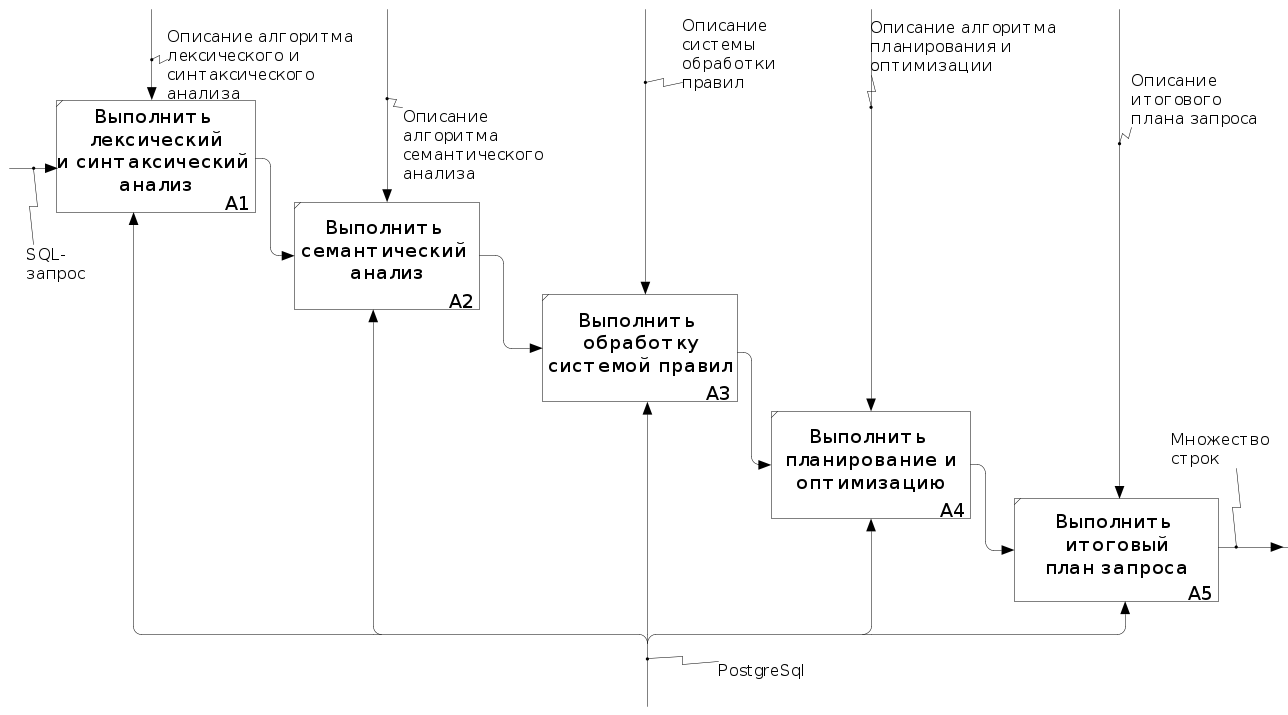
\includegraphics[scale=0.37]{./images/02_A0.png}
		\caption{Выполнение запроса в PostgreSQL.}
	    \label{image:query_plan}
    }
\end{figure}

Основными шагами, которые выполняются при выполнении SQL-запроса в реляционных СУБД являются следующие \cite{stages_sql_query}.

\begin{enumerate}
	\item Лексический и синтаксический анализ. На данном этапе входная строка пользователя обрабатывается лексическим и синтаксическим анализаторами; в результате строится дерево запроса.
	\item Семантический анализ. Полученное на предыдущей стадии дерево запроса дополняется различного рода метаинформацией: системными идентификаторами таблиц, типами и порядковыми номерами запрашиваемых полей, перечнем соединяемых таблиц и т.д.
	\item Обработка системой правил. Далее выполняется поиск в системных каталогах правил, применимых к дереву запроса, и при обнаружении подходящих выполняются преобразования, которые описаны в теле найденного правила. Примером такого преобразования является замена представлений (\textit{виртуальных таблиц}) на обращение к базовым таблицам из определения представления.
	\item Планирование и оптимизация. На вход планировщику поступает структура с деревом запроса (приложение \ref{}). Осуществляется выбор наиболее эффективного пути выполнения этого запроса с точки зрения имеющихся оценок затрат и статической информации на момент выполнения.  После выбора оптимального метода доступа к данным, конечный вариант преобразуется в полноценный план запроса и передается исполнителю. 
	\item Выполнение итогового плана запроса. Исполнителем осуществляется рекурсивный обход по дереву плана: \textit{сканируются отношения}, выполняется \textit{сортировка} и \textit{соединения}, вычисляет \textit{условия фильтра} и др. После выполненных этапов возвращается результирующее множество строк.
\end{enumerate}

\section{План выполнения запроса}
План выполнения запроса действует как дерево инструкций, которым должен следовать механизм выполнения запроса для получения результатов. Он показывает, как будут сканироваться таблицы; если необходимо связывание нескольких таблиц, то какой алгоритм будет выбран для объединения считанных строк.

На примере PostgreSQL работа планировщика запросов для одной таблицы выглядит следующим образом \cite{plan_query_postgres}.
\begin{enumerate}
	\item Выполнение предварительной обработки. 
	\item Оценка всевозможных путей доступа к данным. Оцениваются затраты на последовательный доступ (\textit{seq scan}), сканирование индексов (\textit{index scan}), \textit{bitmap scan}; затем выполняется сортировка (\textit{sort}) или присоединение данных (\textit{join}).
	\item Выбор кратчайшего пути по затратам.
\end{enumerate}

При увеличении числа таблиц, участвующих в запросе, к основному алгоритму добавляются шаги.
\begin{itemize}
	\item Уровень 1. Найти кратчайший путь выполнения запроса для каждой таблицы.
	\item Уровень 2. Получить самый кратчайший путь для каждой комбинации, в которой которой выбирается две таблицы из всех.
	\item Уровень 3. Продолжить ту же обработку, пока в результате число таблиц не станет равным текущему уровню.
\end{itemize}

Процесс получения <<дешевого>> доступа к данным приведен на рисунке \ref{image:data_access}.
\begin{figure}[H]
	\centering
	{
		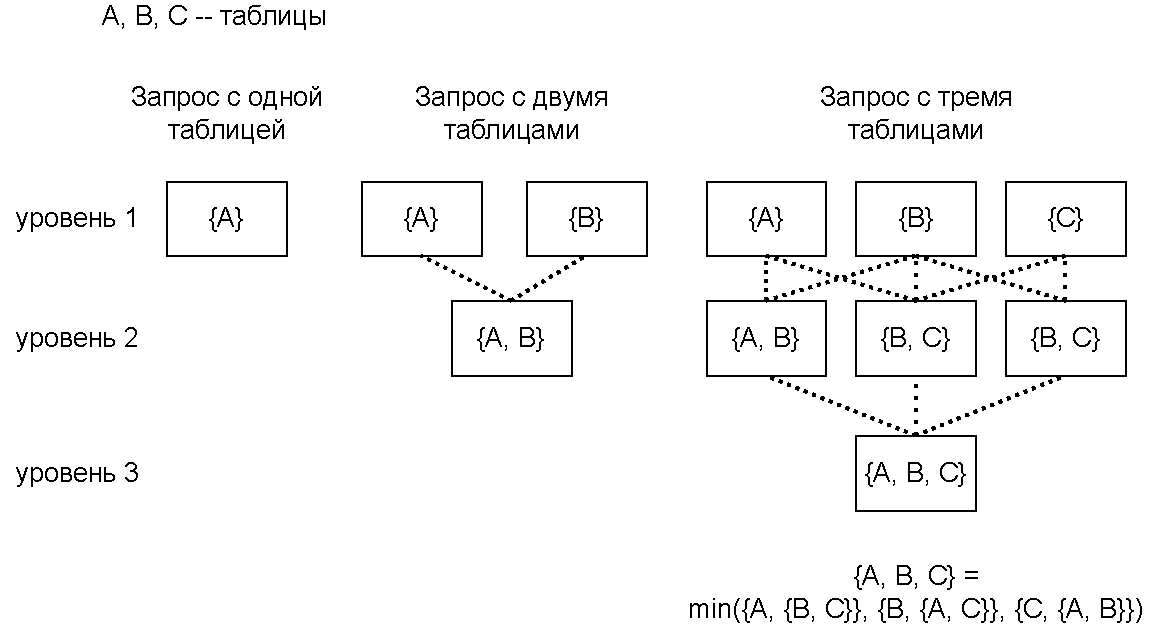
\includegraphics[scale=0.8]{./images/postgre_plan.pdf}
		\caption{Получение <<дешевого>> доступа к данным.}
		\label{image:data_access}
	}
\end{figure}

Для получения оптимального дерева плана запроса, планировщик должен рассмотреть комбинации всех индексов и возможности методов объединения. При увеличении числа используемых таблиц может наступить <<комбинаторный взрыв>>. Таким образом, при количестве таблиц, большем 12, используются \textit{генетические алгоритмы}.

\section{Выбор БД}

\subsection{AdventureWorks}
В качестве базы данных была выбрана <<Adventure Works Cycles>> -- фиктивная компания, разработанная Microsoft для моделирования бизнес-процесса \cite{adventureworks}. Данная фирма <<является>> крупной и многонациональной, которая производит и продает металлические и композитные велосипеды на коммерческих рынках Северной Америки, Европы, Азии.

По своей структуре база данных <<AdventureWorks>> является сложной: состоит из множества схем отношений, соединенных друг с другом различными связями. Диаграмма базы данных этой компании приведена в приложении А.

\subsection{Northwind}
База данных Northwind содержит данные о продажах фиктивной компании под названием “Northwind Traders”, которая импортирует и экспортирует специальные продукты питания со всего мира \cite{northwind}. Диаграмма БД этой компании приведена в приложении Б.

\subsection{Chinook}
Модель данных Chinook представляет собой хранилище цифровых медиа, включая таблицы для исполнителей, альбомов, медиадорожек, счетов-фактур и клиентов \cite{chinook}. Диаграмма БД этой компании приведена в приложении В.

